% !TeX spellcheck = pt_BR
%!TEX root = ../main_text.tex
% !TeX encoding = UTF-8
\chapter{Protótipo de Capacete para Segurança de Ciclistas} \label{chap:prototipo}

    Neste trabalho desenvolveu-se um protótipo de capacete inteligente que realizaria verificações da distância de objetos nas costas do ciclista, alertando-o de possíveis riscos de acidentes.
    Caso esteja em situação de risco, o capacete emitiria sinais visuais luminosos, além do envio de aviso para um segundo dispositivo como um \textit{smartphone} alertando-o de sua situação.
    

    \section{Grafo de Chamada e Códigos Candidatos aos Particionamento}
        
        Como é exibido na Figura \ref{fig:gc}, o grafo de chamada do \wearable\ constitui-se basicamente de leitura das distâncias, cálculo de risco e aviso ao usuário.
        % o que é iteração do wearable
        Cada ciclo completo é considerado uma iteração do sistema \wearable.
        
        \begin{figure}[h] \centering
            \vspace{-0.5em}
            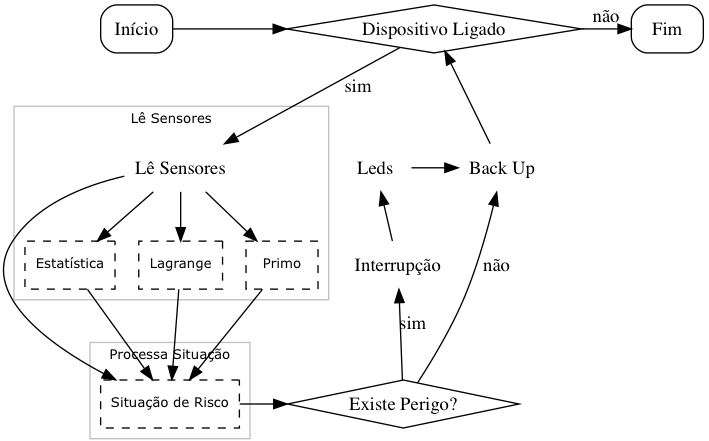
\includegraphics[width=0.65\textwidth]{img/capacete.png}
            \caption{Grafo de chamada do algoritmo base do \wearable. Itens quadriculados exibem a localização dos algoritmos candidatos ao particionamento.}
            \label{fig:gc}
        \end{figure}
        
        O particionamento foi avaliado em duas seções principais, sendo elas a de leitura e de processo de situações, constituindo-se de quatro situações diferentes de particionamento para análise (itens pontilhados na Figura \ref{fig:gc}).
        
        Os algoritmos \A$_{i}$\ candidatos ao particionamento serão:
        
        \begin{itemize}
            \item \A$_{Es}$: Análise Estatística (Algoritmo \ref{alg:statistic}) calculará valores de desvio padrão e variância dos valores no \buffer;
            
            \item \A$_{La}$: Lagrange (Algoritmo \ref{alg:lagrange}) interpolará novas distâncias a partir dos dados do \buffer; 
            \item \A$_{NP}$: Números Primos (Algoritmo \ref{alg:prime}) avaliará se a soma das distâncias lidas correspondem aos números primos;
            %As análises serão feitas por meio de exclusão, selecionando apenas um algoritmo por vez;
            \item \A$_{Ri}$: Processamento de risco (Algoritmo \ref{alg:risk}), na seção de processo de situações.
        \end{itemize}
    
    
        
        %Explicando as implementações de A
        Foi realizado o particionamento para cada algoritmo candidato \A$_{i}$, gerando tanto sua versão em código em nível de \software,\ quando seu módulo em \hardware,\ utilizados para testes comparativos de desempenho.
        
        % s de forma geral
        Para a execução dos testes, todos os \A$ _i $\ em suas versões \hs\ foram executados em implementações sistêmicas sintetizáveis \Ss$ _j $,\ constituídas de módulos como \textit{soft-}processador MicroBlaze, além de memórias, interfaces para comunicação com os dispositivos conectados, entre outros, permitindo o funcionamento completo do \wearable\ \citep{obeidat2011microblaze}.
        
        % as versões de a em software
        Todos os algoritmos \A$_{i}$ em suas versões de \software\ foram executados em uma única implementação \Ss$ _j $, já que esta era compatível com qualquer aplicação em nível de \software, dependendo somente da disposição das instruções na memória.
        Ou seja, para trocar o \A$_{i}$ por \A$_{k}$ neste sistema basta recompilar o projeto em \software.
        Os testes neste sistema serão referenciados como \Ss$ _{s} $.
        
        % algoritmos em hardwares
        % explicando que a necessitam de interfaces
        Algoritmos \A$ _i $\ em \hardware\ também executam em sistemas \Ss$ _j $, mas tais sistemas possuem características ímpares já que são acrescentados módulos sintetizáveis de cada algoritmo.
        %
        Como cada \A$_i$ possui seu próprio módulo, definiu-se um sistema \Ss$_j$ para cada algoritmo \A$_{i}$ em sua versão em nível de \hardware.
        
        Assim, como a Tabela~\ref{tab:bate_o_olho} exibe, \Ss$_s$ é o sistema para testes de todos os algoritmos \A$_{i}$\ em \softwares,\ não possuindo nenhuma adição de implementação sintetizável de \hardwares\ particionados.
        Os outros sistemas são para testes dos módulos dos respectivos algoritmos \A$ _i $ juntos de sua interface de comunicação \hs.
        
%        Dessa forma, os sistemas \Ss$_{j}$ que serão utilizados para teste são:
%        \begin{itemize}
%            \item \Ss$_s$: sistema para testes de todos os algoritmos \A$_{i}$\ em \softwares.
%            Não possui nenhuma adição de implementação sintetizável de \hardwares\ particionados;
%            \item \Ss$_{Es}$: sistema para testes do particionamento em \hardware\ do algoritmo \A$_{Es}$. 
%            Constitui-se do sistema acrescido do módulo sintetizável em \hardware\ \A$_{Es}$ e sua interface de comunicação com o módulo;
%            \item \Ss$_{La}$: sistema para testes do particionamento em \hardware\ do algoritmo \A$_{La}$. 
%            Constitui-se do sistema acrescido do módulo sintetizável em \hardware\ \A$_{La}$ e sua interface de comunicação com o módulo;
%            \item \Ss$_{NP}$: sistema para testes do particionamento em \hardware\ do algoritmo \A$_{NP}$. 
%            Constitui-se do sistema acrescido do módulo sintetizável em \hardware\ \A$_{NP}$ e sua interface de comunicação com o módulo; e
%            \item \Ss$_{Ri}$: sistema para testes do particionamento em \hardware\ do algoritmo \A$_{Ri}$. 
%            Constitui-se do sistema acrescido do módulo sintetizável em \hardware\ \A$_{Ri}$ e sua interface de comunicação com o módulo;
%        \end{itemize}
        
        \begin{table}[h]\centering
            \vspace{-1em}
            %\scriptsize
            %\raaa{1.0}
            \raaa{0.9}
            \caption{Exibição dos Algoritmos Candidatos e os seus Sistemas para Teste}

\begin{tabular}{rc|cp{0.04em}c|cp{0.04em}c|cp{0.04em}c|c}
    \toprule
    & \multicolumn{2}{c}{\A$_{Es}$} && \multicolumn{2}{c}{\A$_{La}$} && \multicolumn{2}{c}{\A$_{NP}$} && \multicolumn{2}{c}{\A$_{Ri}$}\\ %\cmidrule{2-9}
    \cmidrule{2-3} \cmidrule{5-6} \cmidrule{8-9} \cmidrule{11-12}
    Implemen: & \textit{Soft.} & \textit{Hard.} && \textit{Soft.} & \textit{Hard.} && \textit{Soft.} & \textit{Hard.} && \textit{Soft.} & \textit{Hard.} \\ \midrule
    \Ss$_{s}$   & X &   && X &   && X &   && X &   \\ \hline
    \Ss$_{Es}$  &   & X &&   &   &&   &   &&   &   \\ \hline
    \Ss$_{La}$  &   &   &&   & X &&   &   &&   &   \\ \hline
    \Ss$_{NP}$  &   &   &&   &   &&   & X &&   &   \\ \hline
    \Ss$_{Ri}$  &   &   &&   &   &&   &   &&   & X \\
    \bottomrule
\end{tabular}
\label{tab:bate_o_olho}
\end{table}
        
        
        
        
    \subsection{Variações do Protótipo}
        A fim de fazer diferentes testes dos códigos particionados foi construído um protótipo modular para a realização de análises de desempenho sobre cada uma de suas variações.
        Os itens modulares são:
        \begin{itemize}
            \item Número de Sensores de Distância: testes serão realizados com um a três sensores. 
            Não aumenta-se a angulação de percepção, mas sim a exatidão dos dados lidos;
            \item \textit{Buffer} de Cada Sensor de Distância: \buffer\ de dados com tamanho 5, 10 e 15 para processamento das distâncias de cada sensor.
            Representam a quantidade de leituras que serão feitas para cada sensor, armazenando-as num vetor, na qual será utilizado como parâmetro para as operações que serão particionadas.
        \end{itemize}
        Dessa forma, sobre cada código candidato foi realizados testes segundo tais variações, tanto em \hardware,\ quanto em \software.
        %Além da avaliação de desempenho e gasto energético, é possível ter diferentes precisões de distância com tais variações.
        %algos
    
    
    \subsection{Equipamentos e Tecnologias Utilizadas}
        A placa utilizada para sintetização foi uma Arty A7-35T, com 32 mil \luts\ (LuTs) sem um \textit{hard-processor}, ou seja, um controlador/processador físico dedicado.
        Para isso, utilizou-se o sistema \textit{soft-processor} MicroBlaze para processamento do código em \software\ e comunicação com \hardware.
        
        
        Todos os algoritmos foram construídos utilizando-se a ferramenta HLS e incorporados ao projeto base com construções de circuitos digitais assistidos pelo computador.
        A comunicação entre \hs\ foi feita utilizando interface AXI.
        A medição de distância foi realizada com um sensor ultrassônico e a comunicação com um segundo dispositivo que utiliza \textit{Bluetooth Low Energy}.
        
        
    \section{Testes}
        % Explicando os testes
        Para a realização dos testes foi feito um procedimento, tendo como base a Figura \ref{fig:distance}. 
        Como o experimento foi realizado em laboratório, utilizou-se escala de centímetros para as análises.
        
        \begin{figure}[h] \centering
            %\vspace{-0.5em}
            %\includegraphics[width=0.5\textwidth]{img/distance.png}
            \caption{Simulação de aproximações de objetos perante o ciclista segundo suas respectivas áreas de segurança.}
            \label{fig:distance}
        \end{figure}
    
        Cada experimento foi realizado no decorrer de 12 iterações.
        Os principais passos do teste são:
        \begin{itemize}
            \item 
            %
            \textit{Iteração 1:} o ciclista, encontra-se a uma distância de 130 centímetros do objeto, sendo sua situação declarada como segura;
            %
            \item 
            \textit{Iteração 4:} o objeto inicia um movimento de aproximação\footnote{Tanto o movimento de aproximação quanto o de afastamento são realizados manualmente por humanos, simulando a situação real de um ciclista em seu meio.} ao ciclista chegando a ultrapassar o limite mínimo de 30 centímetros. Nisso, a situação do ciclista passa a ser de risco;
            %
            \item
            \textit{Iteração 6:} o objeto ainda encontra-se próximo ao ciclista;
            \item 
            \textit{Iteração 9:} o objeto afasta novamente do ciclista para 130 centímetros, retornando à situação segura;
            \item 
            \textit{Iteração 12:} última leitura para testes, ciclista ainda em situação segura.
            %
        \end{itemize}
    
        As iterações não citadas representam a permanência do estado da iteração anterior à ela.
   
        Este teste foi realizado em cada análise de particionamento com sua variação de módulo. 
        Ou seja, para cada um dos 4 algoritmos, em todas suas variações de sensores e \buffer, um total de 36 situações diferentes para \hs\ serão feitos 30 testes em sequência para cada uma dessas situações, para análises estatísticas de desempenho.
        
        Como a pesquisa tem o objetivo de avaliar o desempenho dos algoritmos candidatos em \hs,\ os tempos de envio de dados e atuação dos sensores foram descartados.
        
        \begin{comment}
        % filtros
        Para que fosse calculado o desempenho do sistema aplicou-se filtros dos quais eliminou-se os seguintes tempos: 
        \textit{a):} o tempo médio gasto da atuação dos sensores; bem como 
        \textit{b):} o tempo de envio para o dispositivo externo. 
        O motivo da filtragem é que o tempo de ambos depende diretamente da sua tecnologia 
        e isso interfere no tempo final.
        %
        Por exemplo, se em determinado teste o objeto ficar um pouco mais distante que 130 centímetros, o tempo da iteração completa será afetado, pois o cálculo depende diretamente da distância.
        O mesmo acontece com a comunicação sem fio, já que não ocorre em tempo constante e, caso falha reenvia-se a informação.
        
        Como o trabalho busca o estudo sobre o desempenho somente sobre a seção de código particionada, eliminou-se estes parâmetros de interferência dos resultados.
        %
        Dessa forma, os valores resultantes à desempenho são os tempos totais $\gamma =\ ^{software}\,/_{hardware} $ sem o tempo de atuação dos sensores e o tempo de envio ao dispositivo, tornando os resultados mais precisos sobre o particionamento.
\end{comment}

        
\chapter{Resultados}   \label{chap:results}
    
    \section{Recursos Alocados para os Algoritmos \A$_{i}$ e Sistemas \Ss$_{j}$}
        %\todo[inline]{Nessa secao atual, a de testes, vc colocara merante uma tabela relacionado os Ss, Aalgoritmo, etc etc etc, de maneira q numa batida de olho de pra entender.}
        %\subsection{Recursos Para Cada Código Candidato \A}      
        
        % tabela hls
        Os valores exibidos pela Tabela \ref{tab:hls} quantificam os recursos utilizados pelo HLS para a geração de cada algoritmo \A$_{i}$ particionado em \hardware.
        
        \begin{table*}[h]\centering
            \vspace{-1em}
            %\scriptsize
            \raaa{1.0}
            %\raaa{0.9}
            \caption{Recursos de FPGA Alocados para cada Código Particionado Utilizando HLS}
            \begin{tabular}{rcc|cc|cc|cc|cc}
                \toprule
                &\multicolumn{2}{c}{Expressões} & \multicolumn{2}{c}{Instâncias}      & \multicolumn{2}{c}{Multiplexadores}  & \multicolumn{2}{c}{Registradores} & \multicolumn{2}{c}{\textit{Total}} \\
                \cmidrule{2-11}
                %\cmidrule{2-3} \cmidrule{5-6} \cmidrule{8-9} \cmidrule{11-12} \cmidrule{14-15}
                & LuTs & F.Fs & LuTs & F.Fs & LuTs & F.Fs & LuTs & F.Fs & LuTs & F.Fs \\
                \midrule
                \A$_{Es}$&52 & 0     & 1948 & 1474   & 364 & 0      & 0 & 394   & 2364 & 1868 \\ 
                \A$_{La}$&128 & 0    & 2048 & 1425   & 309 & 0      & 0 & 479   & 2483 & 1904 \\ 
                \A$_{NP}$&1826 & 0   & 486 & 552     & 236 & 0      & 0 & 527   & 2448 & 1079 \\ 
                \A$_{Ri}$&18 & 0     & 120  & 82     & 15  & 0      & 0 & 34    & 153  & 116  \\ 
                \bottomrule
            \end{tabular}
            \label{tab:hls}
        \end{table*}
        
        
        Em cada linha exibe-se os valores de alocação referentes a cada algoritmo, sendo os algoritmos Estatístico \A$_{Es}$, Lagrange \A$_{La}$, Números Primos \A$_{NP}$ e Risco \A$_{Ri}$.
        %Já as colunas exibem para quais propósitos determinados recursos em \hardware\ foram utilizados, na qual expressões representam recursos em \hardware\ para cálculos lógico/matemáticos, instâncias para memorização de recursos utilizados nas expressões, assim como as alocações de multiplexadores e registradores para fins mais específicos\todo{melhorar}.
        Já as colunas exibem para quais propósitos determinados recursos em \hardware\ foram utilizados, na qual são expressões, instâncias, multiplexadores e registradores, todos formados das tecnologias de \luts\ e \ffs.       
        %
        Na última coluna é contabilizado o total de gastos de cada \hardware\ gerado.
        
        %Linkando a com b
        %Com cada o módulo particionado gerado, deve-se então adicioná-los aos respectivos sistemas.
        
        
        
        %\subsection{Recursos Para Cada Sistema \Ss}
        
        A Tabela~\ref{tab:vivado} exibe os valores de alocação e gasto energético sobre cada sistema \Ss$_{j}$ utilizado para teste.
        
        \begin{table}[h]\centering
            \vspace{-1em}
            %\scriptsize
            %\footnotesize 
            \raaa{1.0}
            %\raaa{0.9}
            \caption{Recursos e Gastos Energéticos Utilizados em todos os Sistemas Completos}
            \begin{tabular}{rcccc}
                \toprule
                & \lut   & \lut\textit{RAM} & \ff             & \textit{Chip Power} \\
                \cmidrule{2-5}
                
                \textit{Disponível}& \textit{20800}  & \textit{9600}              & \textit{210}     & -      \\\cmidrule{1-5}
                \Ss$_{s}$ & 11991  & 1781              & 11612           & 0,922W \\
                \Ss$_{Es}$& 13640  & 1822              & 13080           & 0,972W \\ 
                \Ss$_{La}$& 13502  & 1808              & 13193           & 0,968W \\ 
                \Ss$_{NP}$& 12959  & 1782              & 12559           & 0,933W \\
                \Ss$_{Ri}$& 12109  & 1781              & 11742           & 0,929W \\ 
                \bottomrule
            \end{tabular}
            \label{tab:vivado}
        \end{table}
    
        As informações exibidas pelas colunas descrevem alocação de \luts, \ffs\ e \luts RAM e o gasto energético médio (\textit{Chip Power}) de cada um dos sistemas \wearables\ testados no protótipo.
        O valor total de recursos disponíveis pela plataforma FPGA é exibido na primeira linha e as demais o valor alocado segundo cada sistema.
        
        \subsection{Análises dos Recursos Utilizados}
    
            Com os valores exibidos por ambas as tabelas, é possível fazer análises de recursos utilizados tanto para os módulos de maneira isolada, quanto para o sistema como um todo.
            Assim, percebeu-se que:
    
    
       %\section{Análise sobre Quantidade de Recursos Alocados e Gasto Energético}
            %Analisando as Tabelas~\ref{tab:hls} e \ref{tab:vivado}, é possível ver que:
            
            \begin{itemize}
                \item 
                % codigo que gastou mais recurso
                O algoritmo de Lagrange \A$_{La}$ é o módulo particionado que utiliza mais recursos dentre todos.
                %Utilizou $8,1\%$ e $4,5\%$ do total disponível pela plataforma FPGA, sendo $18,3\%$ de \lut\ e $14,4\%$ de \ff\ do projeto final;
                Mesmo assim, ao incorporar os códigos particionados aos sistemas, seu sistema (\Ss$_{La}$) não foi o maior em utilização de recursos de FPGA;
                
                \item
                %sistema que mais gastou recursos
                A maior diferença na utilização de recursos entre sistemas completos, comparando totalmente em \software\ com sistemas com módulos particionados em \hardware,\ é de $5,5\%$, na qual foi sobre as partições do algoritmo candidato Estatístico \Ss$_{s}$ e \Ss$_{Es}$, \software\ e \hardware\ respectivamente. 
                Isso pois, enquanto o \Ss$_{s}$ utilizou $45,3\%$ do total de \luts\ disponíveis (ambas \luts\ e \luts RAM) para a confecção do sistema no FPGA, \Ss$_{Es}$ que inclui o múdulo em \hardware,\ utilizou $50,8\%$.
                
                Essa diferença entre recursos alocados também está presente na forma em que a interface de comunicação está sendo utilizada em seus módulos.
                Mesmo \A$_{Es}$ não sendo o maior módulo, seu sistema \Ss$_{Es}$ foi, indicando que a construção de sua interface de comunicação requisitou grande quantia de recursos;
                
                \item
                Comparando o gasto energético dos sistemas particionados com o sistema em \software, o maior gasto também é de \Ss$_{Es}$, necessitando de $5,4\%$ Watts a mais que \Ss$_{s}$. \\
                O sistema com o módulo Lagrange em \hardware\ (\Ss$_{La}$) teve a menor diferença, utilizando $0,7\%$ Watts a mais que \Ss$_{s}$.
            \end{itemize}
               
           

    \section{Desempenho}
    
        A Figura \ref{fig:desempenho} exibe os valores obtidos das análise de desempenho entre \hs\ (conforme apresentado na Seção \ref{sec:ganho_desempenho}).
        Mostra-se todos os algoritmos separados em quadros, bem como suas variações de sensores e \buffer.
        
        No eixo das abscissas tem-se \textit{Sen} e \textit{Buf} representando a variação de sensores e do tamanho de \buffer\ no protótipo, respectivamente.
        Já no eixo das ordenadas exibe-se o valor performático dos 30 testes para cada uma das 36 situações, segundo a Equação~\ref{eq:soft_hard}.
        
        \begin{figure*}[h] \centering
            \vspace{-0.5em}
            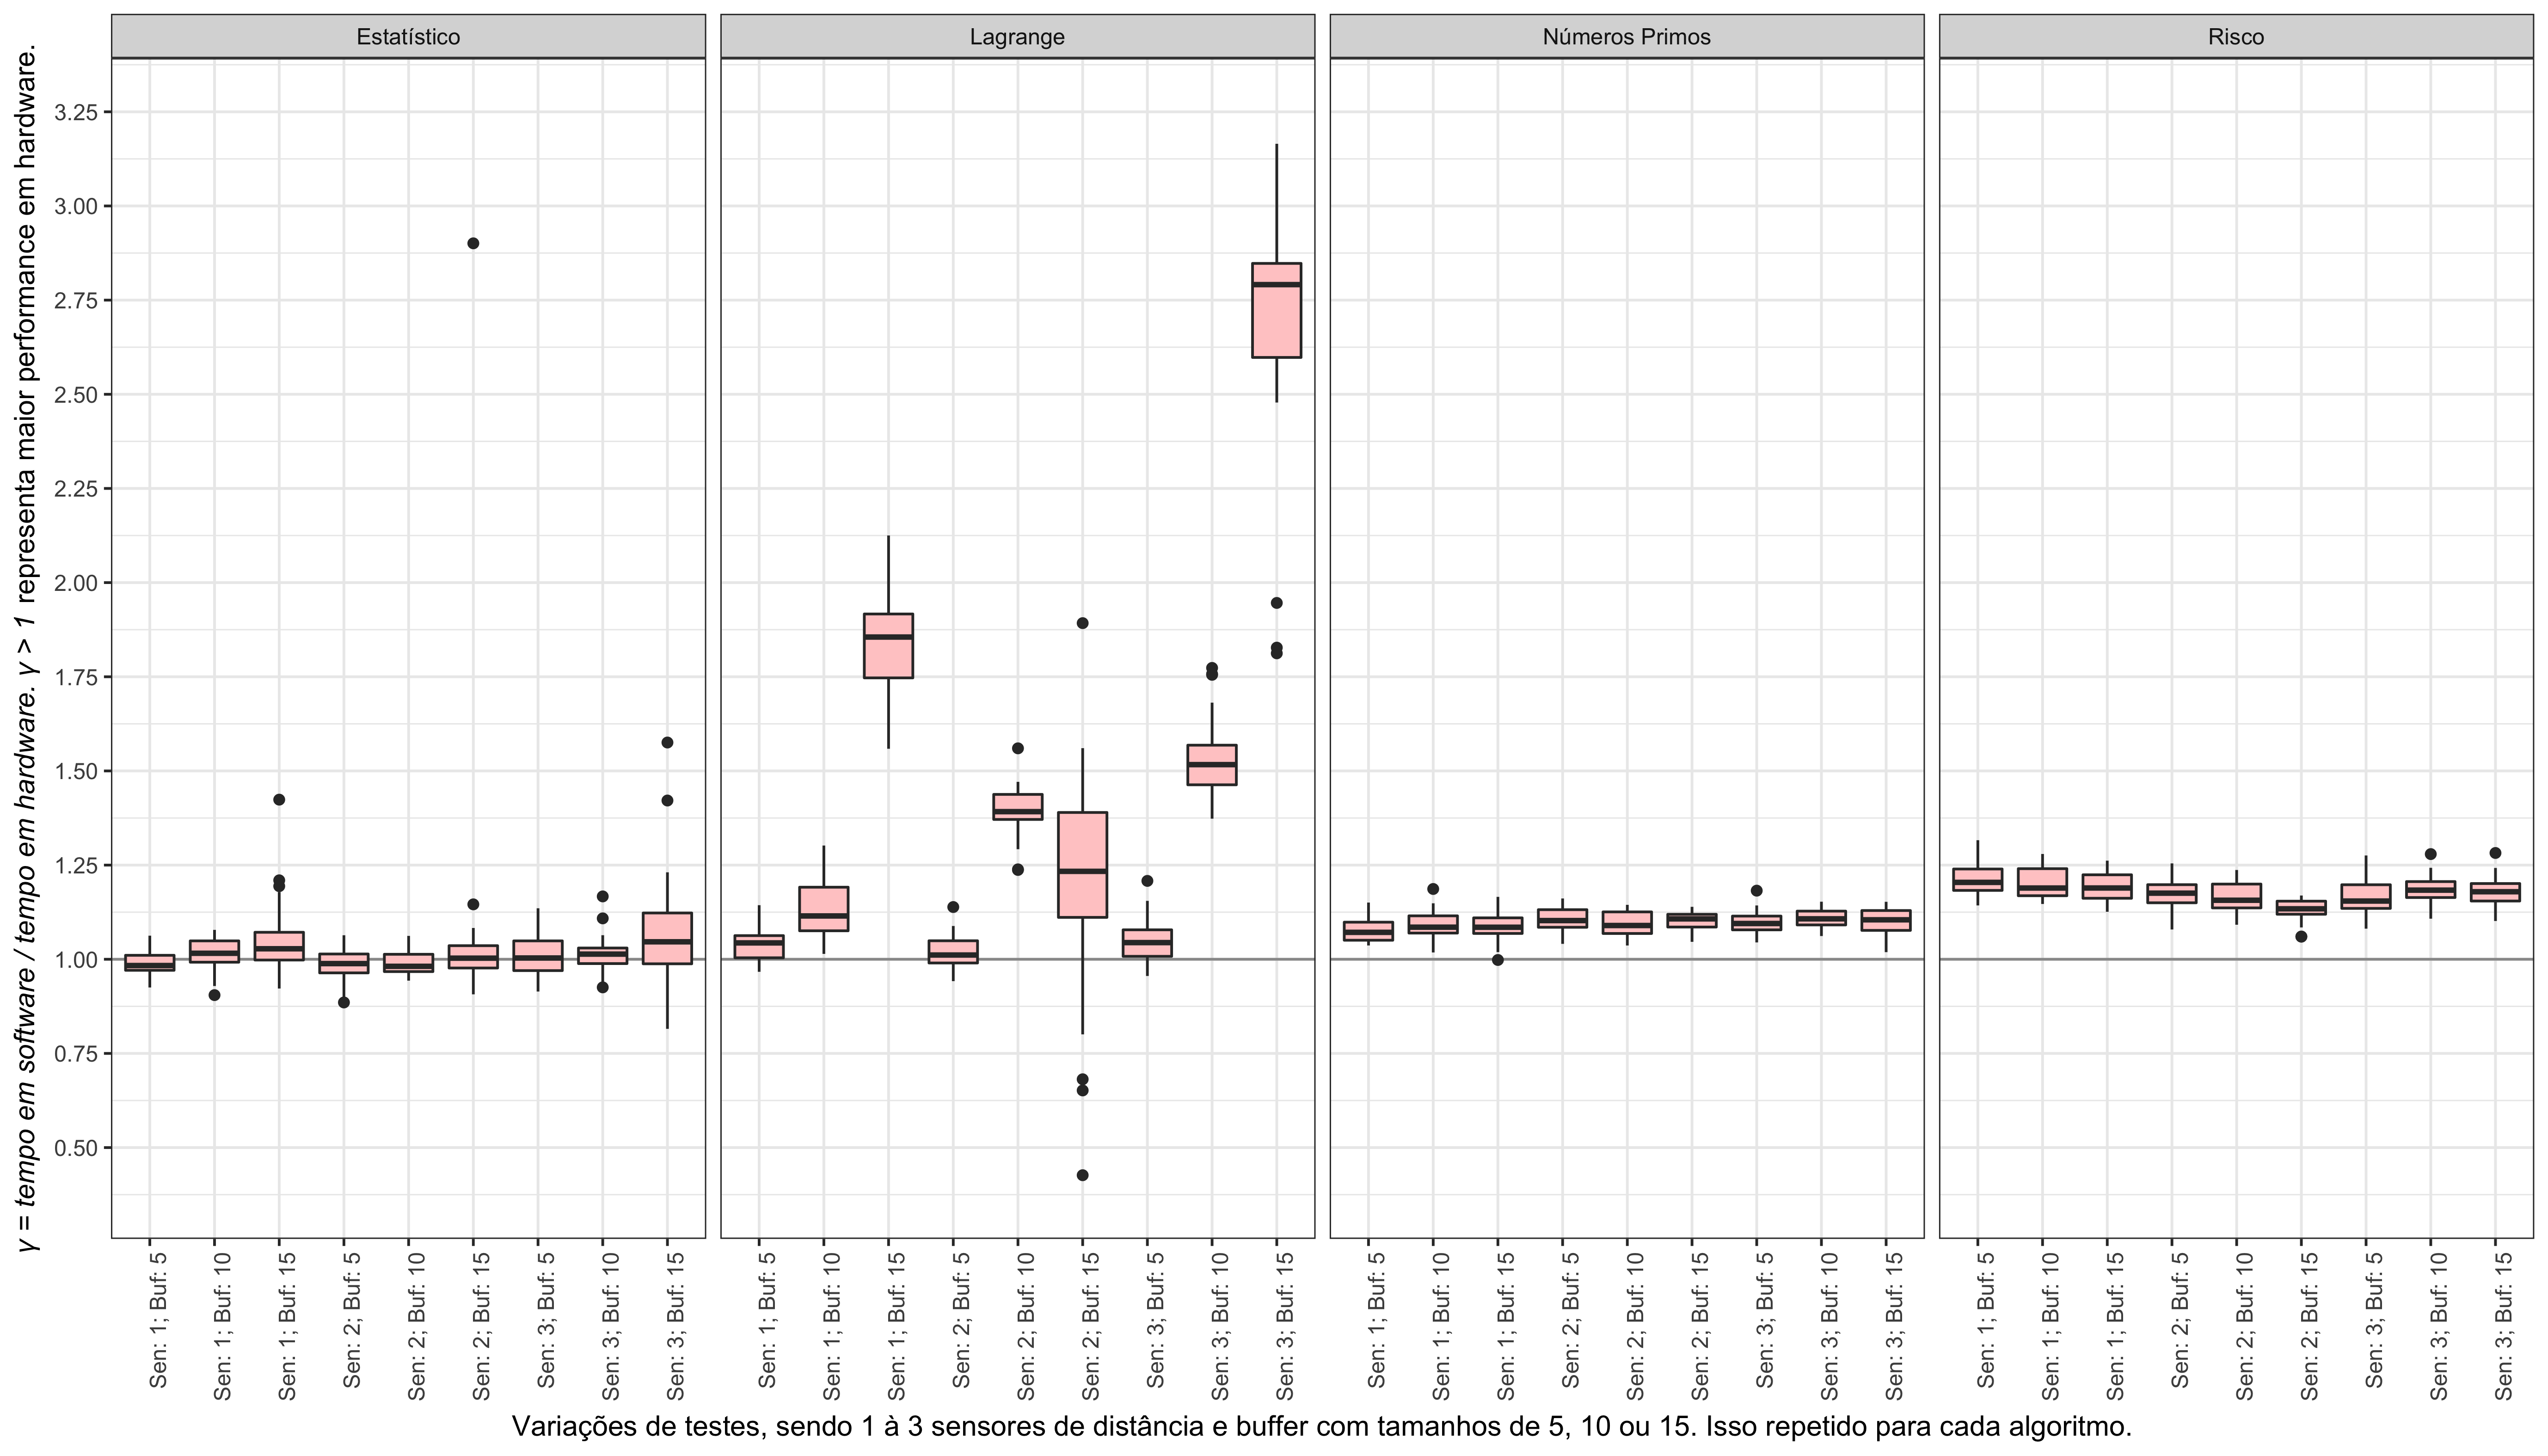
\includegraphics[width=1\textwidth]{img/performance.png}
            \caption{Gráfico com os valores performáticos de uma das 36 variações de protótipo, separados por código candidato. Valores de $\gamma > 1.0 $ exibem maior desempenho no \hardware\ particionado.}
            \label{fig:desempenho}
        \end{figure*}
   
    
        Além da Figura~\ref{fig:desempenho}, os valores médios também podem ser lidos pela Tabela~\ref{tab:desempenho}.
        Cada linha desta representa um quadro da Figura~\ref{fig:desempenho}.
        Como complemento, na última coluna tem-se uma média de desempenho de cada algoritmo em todas as suas variações de teste.
        
        \begin{table}[h]\centering
            %\vspace{-1em}
            %\scriptsize
            \raaa{1.0}
            %\raaa{0.9}
            \caption{Médias das Análises Performáticas em suas Variações}
            \begin{tabular}{rccc|ccc|ccc|c}\toprule
                & \multicolumn{3}{c}{1 Sensor} & \multicolumn{3}{c}{2 Sensores} & \multicolumn{3}{c}{3 Sensores}& \\
                \cmidrule{2-11}
                \textit{Buffer} & 5 & 10 & 15 & 5 & 10 & 15 & 5 & 10 & 15 & $\bar{x}$ \\
                \midrule
                \Ss$_{Es}$   & 0.989 & 1.013 & 1.052  & 0.982 & 0.992 & 1.069  & 1.009 & 1.011 & 1.08  & 1.022 \\
                \Ss$_{La}$   & 1.036 & 1.132 & 1.844  & 1.019 & 1.395 & 1.14   & 1.046 & 1.37  & 2.765 & 1.416 \\
                \Ss$_{NP}$   & 1.076 & 1.092 & 1.084  & 1.105 & 1.094 & 1.103  & 1.099 & 1.109 & 1.102 & 1.096 \\ 
                \Ss$_{Ri}$   & 1.212 & 1.203 & 1.195  & 1.17  & 1.161 & 1.132  & 1.168 & 1.183 & 1.179 & 1.178 \\
                \bottomrule
            \end{tabular}
            \label{tab:desempenho}
        \end{table}
        
        
        \subsection{Análises de Desempenhos}
        %Análise de desempenho
        % quase todos foram suuuuuuuucesssooooooooo 
        Os resultados mostram que:
        \begin{itemize}
            \item 
            Os sistemas com Número Primo e Risco (\Ss$_{NP}$ e \Ss$_{Ri}$) obtiveram um ganho de desempenho considerável e estável, comparado com suas versões não particionadas, sendo em média $9,6\%$ e $17,8\%$ mais eficiente em suas obrigações;
            
            \item 
            Mesmo com o sistema Lagrange (\Ss$_{La}$) exibindo resultados não-estáveis nas variações como os de \Ss$_{NP}$ e \Ss$_{Ri}$, $87\%$ dos testes realizados obtiveram maior desempenho em \hardware.
            A média final de desempenho desde sistema superou a versão em \software\ em $41,6\%$;
            
            \item 
            O algoritmo Estatístico (\Ss$_{Es}$) obteve três situações de variação de protótipo na qual não utilizar o particionamento resultava em maior desempenho, sendo seu desempenho $45,5\%$ iguais ou melhores para o sistema totalmente em \software.
            %são (1; 5), (2; 5) e (2; 10) sendo números de sensores e tamanho de \buffer\ respectivamente.
            As variações que \software\ obteve mais desempenho foram: [\textit{Sen} 1; \textit{Buf} 5], [\textit{Sen} 2; \textit{Buf} 5] e [\textit{Sen} 2; \textit{Buf} 10]. 
            Entretanto, a média dos resultados de todas as variações de protótipos mostram que ainda assim esse sistema foi $2,2\%$ mais eficiente em \hardware\ que \software.
        \end{itemize}
    
    
        %\item 
        % Achismos
        O baixo resultado do sistema \Ss$_{Es}$ já era esperado, pois este e todos os outros algoritmos não receberam nenhuma otimização em \hardware,\ nem em sua interface de comunicação.
        O algoritmo Estático especificamente (Algoritmo \ref{alg:statistic}), é o único que realiza mais de uma leitura sobre os dados de \buffer\ disponibilizados via parâmetro, sendo as operações situadas nas linhas 3 e 5.
        Este algoritmo é custoso computacionalmente, pois o uso de cada elemento de \buffer\ requer também uma comunicação entre \hs,\ solicitando o respectivo dado, criando uma sobrecarga no barramento e, consequentemente, a queda de desempenho pela sua espera.
        
        %resolvendo o problema
        Este problema pode ser contornado de várias formas.
        A mais simples seria utilizar uma memória interna no \hardware\ extra que, após a cópia de todos os valores do \buffer, pode-se operar lendo da sua própria memória.
        \textit{Pipeline}, \textit{unroll} de \textit{loops} e protocolos de comunicação adequados são tipos de otimizações mais complexas, mas que poderiam resultar em melhora de desempenho, não aplicando só ao Estatístico, mas também todos os outros.
        
        
\begin{comment}


\begin{table}[h]\centering
\vspace{-1em}
\scriptsize
%\raaa{1.0}
\raaa{0.9}
\caption{Diferença Performática entre os Particionamentos par cada Conjunto de 12 Iterações do Wearable}
\begin{tabular}{@{}R{1.3em}R{1.6em}R{1.5em}R{1.5em}|R{1.6em}R{1.6em}R{1.6em}|R{1.5em}R{1.5em}R{1.5em}|c@{}}\toprule
& \multicolumn{3}{c}{1 Sensor} & \multicolumn{3}{c}{2 Sensores} & \multicolumn{3}{c}{3 Sensores}& \\
\cmidrule{2-11}
\textit{Buf} & 5 & 10 & 15 & 5 & 10 & 15 & 5 & 10 & 15 & $\bar{x}$ \\
\midrule
\Ss$_{Es}$   & -2.0   &    0.5  &    0.4  &   -2.7  &   -1.6  &   -1.8  &    0.4  &   0.3   &     4.2   & -0.2 \\
\Ss$_{La}$   &  7.7   &    9.3  &    8.6  &   10.9  &    9.9  &   11.6  &   10.2  &   12.0  &    12.1   & 10.2 \\
\Ss$_{NP}$   &  2.8   &   12.2  &   91.8  &    1.6  &   44.6  &   13.9  &    4.1  &   64.8  &   231.3   & 51.9 \\
\Ss$_{Ri}$   & 17.8   &   17.2  &   16.9  &   15.0  &   14.9  &   12.9  &   15.0  &   17.5  &    18.4   & 16.1 \\
\bottomrule
\end{tabular}
\label{tab:iterationsmilissegundos}
\end{table}


Power bigger  5,4229934924
Power little  0,7592190889

hls1 ao todo lt 7,7763157895
hls1 ao todo ff 4,4903846154

hls1 ao projeto lt 17,3313782991
hls1 ao projeto ff 14,2813455657

hls2 ao todo lt 8,1677631579
hls2 ao todo ff 4,5769230769

hls2 ao projeto lt 18,3898681677
hls2 ao projeto ff 14,4318957023

maior projeto lut 65,5769230769  ram 18,9791666667      lut all 50,8618421053    ff 31,7139423077             chip
software lut 57,6490384615       ram 18,5520833333      lut all 45,3026315789    ff 27,9134615385             chip

    Expression & Instance      & Multiplexer  & Register & Total
    52 / 0     & 1948 / 1474   & 364 / 0      & 0 / 394   & 2364 / 1868 \\ statistic
    128 / 0    & 2048 / 1425   & 309 / 0      & 0 / 479   & 2483 / 1904 \\ lagrange
    1826 / 0   & 486 / 552     & 236 / 0      & 0 / 527   & 2448 / 1079 \\ prime
    18 / 0     & 120  / 82     & 15  / 0      & 0 / 34    & 153  / 116  \\ risk
    
    
    & LUT    & LUTRAM   & FF     & IO     & On-Chip Power & Power supplied to off-chip devices
    & 20800  & 9600     & 41600  & 210    & -             & - \\
    & 13640  & 1822     & 13080  & 104    & 0,972         & 0,506 \\ statistic
    & 13502  & 1808     & 13193  & 104    & 0,968         & 0,506 \\ lagrange
    & 12959  & 1782     & 12559  & 104    & 0,933         & 0,506 \\ prime
    & 12109  & 1781     & 11742  & 104    & 0,929         & 0,506 \\ risk
    
    (-2,0   +    0,5  +    0,4  +   -2,7  +   -1,6  +   -1,8  +    0,4  +   0,3   +     4,2) / 9 = -0.2
    ( 7,7   +    9,3  +    8,6  +   10,9  +    9,9  +   11,6  +   10,2  +   12,0  +    12,1) / 9 = 10.2
    ( 2,8   +   12,2  +   91,8  +    1,6  +   44,6  +   13,9  +    4,1  +   64,8  +   231,3) / 9 = 51.9
    (17,8   +   17,2  +   16,9  +   15,0  +   14,9  +   12,9  +   15,0  +   17,5  +    18,4) / 9 = 16.1
    
\end{comment}


\begin{comment}
    \begin{table}\centering
    \scriptsize
    \raaa{1.3}
    \caption{Cálculo de desempenho sobre variações em I/O e algoritmo particionado.}
    \begin{tabular}{@{}rrrrcrrrcrrr@{}}\toprule
    & \multicolumn{3}{c}{$\mathcal{O}(1)$} && \multicolumn{3}{c}{$\mathcal{O}(n)$} & & \multicolumn{3}{c}{$\mathcal{O}(n\log n)$}\\
    \cmidrule{2-4} \cmidrule{6-8} \cmidrule{10-12}análise& 5 & 10 & 15 && 5 & 10 & 15 &&5 & 10 & 15 \\
    \midrule \textit{sistêmica} \\
    %média     & ? & ? & ? && ? & ? & ? && ? & ? & ? \\
    $\bar{x}$     & ? & ? & ? && ? & ? & ? && ? & ? & ? \\
    $\sigma^2$ & ? & ? & ? && ? & ? & ? && ? & ? & ? \\
    $\sigma$ & ? & ? & ? && ? & ? & ? && ? & ? & ? \\
    \midrule \textit{empírica} \\
    %média     & ? & ? & ? && ? & ? & ? && ? & ? & ? \\
    $\bar{x}$     & ? & ? & ? && ? & ? & ? && ? & ? & ? \\
    $\sigma^2$ & ? & ? & ? && ? & ? & ? && ? & ? & ? \\
    $\sigma$ & ? & ? & ? && ? & ? & ? && ? & ? & ? \\
    \bottomrule
    \end{tabular}
    \end{table}
    \end{frame}
\end{comment}



\chapter{Conclusões} \label{chap:conclu}
    %projeto de sistemas
    A demanda por curto tempo para disponibilidade ao mercado, somado ao fato dos produtos exigirem propriedades de corretude, rapidez, confiabilidade e preço acessível representam um desafio para projetistas de sistemas embarcados em geral.
    %utiliza o particionamento para o problema de desempenho
    Com o desenvolvimento de sistemas embarcados cada vez mais complexos, o particionamento \hs\ tornou-se um problema de otimização em \codesign\ de sistemas.
    %wearable
    Como dispositivos \wearables\ também demandam um alto desempenho e/ou baixo consumo de energia sem apresentar desequilíbrio em confiabilidade e segurança entre outros, aplicou-se o particionamento sobre essa classe de sistemas, com foco em tais melhorias.
    
    %proposta
    A proposta da pesquisa constituiu-se na busca pelo aprimoramento de desempenho de dispositivos computacionais \wearables,\ utilizando o particionamento como meio, visando gasto energético e de recursos limitados de plataforma FPGA.
    
    %comentando os testes
    Para a avaliação, realizou-se particionamento de quatro algoritmos candidatos (Estatístico \A$_{Es}$, Lagrange \A$_{La}$, Números Primos  \A$_{NP}$ e Processamento de Risco \A$_{Ri}$) de um projeto de capacete de segurança para ciclistas, variando cada teste em quantidade de sensores e também o \buffer\ de operação.
    
    % comentando os resultados
    Três dos quatro sistemas (Lagrange \Ss$_{La}$, Números Primos \Ss$_{NP}$ e Risco \Ss$_{Ri}$) obtiveram sucesso na busca por desempenho apenas pelo processo de particionamento, aumentando no mínimo $9,6\%$ seus desempenhos, utilizando o valor máximo de $ 5,5\% $ de recursos e $ 5,4\% $ de energia do \hardware\ reconfigurável.
    %
    O sistema Estatístico \Ss$_{Es}$ em $45,5\%$ dos testes obteve maior desempenho \software\ comparado com \hardware.
    Esse resultado já era esperado, já que seu código exige bastante comunicação entre \hs, afetando seu desempenho.
    
    %trabalhos futuros
    %har e softprocessadores
    Para futuros trabalhos seria possível realizar a comparação do sistema \wearable\ particionado variando, também a arquitetura de sintetização, ou seja, testes de desempenho entre \textit{soft} e \textit{hard-}processadores, ambos utilizando FPGA.
    
    % fpga e prototipações
    %Comparações entre o uso de plataformas FPGA e plataformas de prototipações também seriam viáveis, ainda com foco em busca em otimizações em desempenho e eficiência energética sobre \wearables.
    
    %mais alguma sugestão de trabalhos?
    %E também a adição do parâmetro otimização em \hardware,\ verificando o percentual de ganho ao utilizar as técnicas de otimizações em nível de \hardware\ existentes para HLS.
    
    
    % use section* for acknowledgment
    %\section*{Agradecimentos} \todo{a}
        %Agradecemos à Universidade Federal de Ouro Preto, ao CNPq, CAPES e à FAPEMIG pelo subsídio dessa pesquisa.        
        
        % conference papers do not normally have an appendix
        %\section*{Apêndice}    
        %    \hphantom{a}
